%!TEX root = ../thesis.tex
%*******************************************************************************
%****************************** Third Chapter **********************************
%*******************************************************************************

\newcommand\independent{\protect\mathpalette{\protect\independenT}{\perp}}
\def\independenT#1#2{\mathrel{\rlap{$#1#2$}\mkern2mu{#1#2}}}


\chapter{Nonlinear Independent Component Analysis}\label{chapter:ica}

% **************************** Define Graphics Path **************************
\ifpdf
    \graphicspath{{Chapter4/Figs/Raster/}{Chapter4/Figs/PDF/}{Chapter4/Figs/}}
\else
    \graphicspath{{Chapter4/Figs/Vector/}{Chapter4/Figs/}}
\fi

\emph{This chapter is largely based on the paper:}

\begin{quote}
	\fullcite{gresele2019incomplete_fullcite}.
\end{quote}

%\emph{The Incomplete Rosetta Stone Problem: Identifiability Results for Multi-View Nonlinear ICA} published at UAI 2019.


\section{Introduction}

%\begin{itemize}
%	\item What is ICA?
%	\begin{itemize}
%		\item cocktail party problem with two speakers
%	\end{itemize}
%	\item Formal definition and definition of identifiability
%	\item Without making assumptions, identifiability is impossible (refer to nonlinear ica section for result)
%	\item Assumptions can be made on the mixing function or on the distribution of sources.
%	\item Discuss ambiguities at high level (identifiability usually is done up to 'tolerable ambiguities')
%\end{itemize}

Independent Component Analysis (ICA) is often motivated by the so-called \emph{cocktail-party problem}.
When two conversations at a party are happening simultaneously, a listener will hear different mixtures of the two audio streams produced by the speakers in each of their ears.
Despite both ears receiving mixtures of the conversations, the listener is able to focus on either of the conversations separately, hearing and understanding one while ignoring the other.
This is due to the brain's ability to separate out the mixed audio streams into the separate underlying sources, one for each conversation.

More generally, given data that are mixtures of independent underlying sources, the goal of ICA is `unmix' the data, thus recovering the sources.
This provides a principled approach to disentanglement of independent latent components, blind source separation, and feature extraction~\citep{hyvarinen2000independent}.
The applications of ICA are ubiquitous, including neuroimaging~\citep{mckeown1998independent}, signal processing~\citep{sawada2003direction}, text mining~\citep{honkela2010wordica}, astronomy~\citep{nuzillard2000blind} and financial time series analysis~\citep{oja2000independent}.

The ICA problem can be written formally by defining the 
latent variable model
%generative model
%\begin{align}
%\bm{x} &= \bm{f}(\bm{s}) \label{eqn:ica-basic-1}\\
%p(\bm{s}) &= \prod_{i} p_i(s_i) \label{eqn:ica-basic-2}
%\end{align}
%
\begin{align}
Z &\sim p(z) = \prod_i p(z_i) \label{eqn:ica-basic-1} \\
%Z &\sim P_Z = \prod_i P_{Z_i}  \\
X &= f(Z) \label{eqn:ica-basic-2}
%p(z) &= \prod_i p(z_i)
\end{align}
%
where $Z$ is a vector of independent \emph{sources}, $X$ is a vector of \emph{observations} or \emph{mixtures} and $f$ is the vector of \emph{mixing functions} expressing how each coordinate of $X$ depends on all of the coordinates of $Z$. 
Given a dataset of observations of $X$, the goal of ICA is to recover the corresponding unknown values of $Z$ by learning to invert the unknown $f$.
In the general case, no assumptions are made about $p(z)$ other than that it factorises.
The latent variable model in this setting should thus be thought of as a true descriptive model for the world, 
in contrast to generative modelling, where latent variable models with factorised priors merely provide a convenient way to specify distributions over the observable variables. 


%where $\bm{s}$ is a vector of independent \emph{sources}, $\bm{x}$ are the vector of \emph{observations} or \emph{mixtures} and $\bm{f}$ is the vector of \emph{mixing functions} expressing how each coordinate of $\bm{x}$ depends on all of the coordinates of $\bm{s}$. 
%%Generally, it is assumed that the number of sources and observations (i.e. the dimension of $\bm{s}$ and $\bm{x}$ respectively) are equal, which we will take to be the case throughout this chapter unless specified otherwise. 
%%If there are more observations than sources, the problem is called \emph{overdetermined} or \emph{undercomplete}, while if there more sources than observations it is called \emph{underdetermined} or \emph{overcomplete} \cite{citation_needed}.
%Given a dataset of observations of $\bm{x}$, the goal of ICA is to recover the corresponding unknown values of $\bm{s}$ by learning to invert the unknown $\bm{f}$.

An ICA problem is known as \emph{identifiable} when it is possible to recover the sources $Z$ up to tolerable ambiguities. 
For instance, it is generally acceptable to recover $Z$ up to linear rescaling or permuted coordinates.
Although identifiability results generally assume access to unlimited samples of data, they are crucial to ensuring the reliability of ICA methods in practical scenarios; in the absence of these, there is no guarantee that a proposed method will successfully reconstruct the true sources, even in controlled settings.

It was proven by \cite{hyvarinen1999nonlinear} that the `vanilla' ICA setting, in which only independence of the sources and invertibility of $f$ are assumed, is \emph{non-identifiable}.
Thus, much of the research in this field has attempted to characterise the assumptions under which identifiability holds.
Such assumptions may be made either on the mixing functions or on the distributions of the sources. 

The central contribution of the work presented in this chapter is the derivation of identifiability results in a novel \emph{multi-view} setting, in which multiple observations of the same underlying sources through different mixing functions are given (see Figure ??\footnote{\todo{Make figure with ICA model and multi-view model side by side to visually explain the setting of this work simply.}}):
%
\begin{align*}
Z &\sim \prod_i p(z_i) \\
X^1 &= f^1(Z) \\
X^2 &= f^2(Z)
\end{align*}
%
In this setting, identifiability holds subject to much weaker assumptions than are required for the single-view setting.
These results are of practical importance for applications in which multiple data modalities may be simultaneously available.

For a high-level intuition of the results, consider the perception of 3D structure through eyesight.
Each of our eyes only sees a 2D projection of the true state of the 3D world.
With only a single eye available, it may be possible to infer the 3D structure present in a scene by exploiting known cues, such as the objects in the scene being familiar to the viewer or the presence of shadows.
But with two eyes together, a human can perceive 3D structure immediately, even without such cues. 
Analogously, the results presented in this work show that inference of latent structure can be performed under much weaker assumptions when more than a single view is available.


The remainder of this chapter is structured as follows.
Section \ref{sec:ica-literature-overview} provides an introduction to ICA and the literature surrounding it, as well as literature from other areas that is relevant to the setting considered in this work.
Section \ref{sec:ica-nonlinear-ica-with-mulitple-views} presents the main results.
Section ?? discusses the assumptions we make, and Section ?? concludes.


%In the rest of this section we give an overview of the different cases for which identifiability results are known. 
%%Note that the ICA literature also includes a variety of methods for implementing solutions to the problem with real data, as well as a variety of application areas. 
%%Since the contribution of this chapter is to prove identifiability results in a novel setting, only the essentials required to understand the novel results in full context will be provided in this section.
%In brief, the case of linear mixing functions has been extensively studied and is well understood, while the non-linear case is more challenging.
%Recently, many papers have used a novel proof technique to derive identifiability results in slight modifications to the standard ICA problem setting.
%The contribution of this chapter (Sections ??-??) is similar, proving identifiability in the case of \emph{multiple nonlinear views}. 
%That is, the given dataset consists of observations $\bm{x}^{(1)}$ and $\bm{x}^{(2)}$ of the same sources $\bm{s}$.

%\emph{Notation: discuss use of bold lower case letters for vectors in usual ICA literature and that here we use capitals for consistency with rest of thesis.}

\section{Overview of ICA and related literature}\label{sec:ica-literature-overview}

This section provides an overview of different ICA settings for which identifiability results are known, and discusses other literature relevant to the multi-view setting considered in this work.


%Sections \ref{subsec:ica-literature-linear-ica} - \ref{subsec:ica-literature-nonlinear-ica-with-aux} provide an overview of different ICA settings for which identifiability results are known.
%In brief, the linear case has been extensively studied and is well understood, while the nonlinear case is more challenging.
%Recently, a novel proof technique has been used to derive identifiability results in slight modifications to the standard ICA problem setting.
%Section \ref{sec:related-work} discusses other literature that is not about ICA but is nonetheless relevant to the setting considered in this work.



\subsection{Linear ICA}\label{subsec:ica-literature-linear-ica}

%\begin{itemize}
%	\item The linear case has been studied extensively and is identifiable if at most one of the components is Gaussian
%	\item If more than one component is Gaussian, then these components cannot be unmixed since Gaussians are closed under linear mixing, so any linear unmixing function will not be able to distinguish them.
%	\item Overview of techniques
%\end{itemize}

\emph{Linear ICA} refers to the setting in which the vector of mixing functions $f$ is a linear map, 
in which case the ICA model can be written
%
\begin{align*}
Z &\sim \prod_i p(z_i) \\
X &= AZ
\end{align*}
%
where $A$ is a square matrix.
This problem has been extensively studied and has been shown to be identifiable if at most one of the latent components is Gaussian~\citep{darmois1953analyse, skitovich1954linear, comon1994independent}.
Nonidentifiability in the case of more than one Gaussian component is a consequence of the fact that an isotropic Gaussian is invariant under orthogonal linear mappings.
Thus if the diagonal matrix $\Lambda$ rescales the Gaussian components of $Z$ to be unit variance, and $U$ is an orthogonal matrix mixing these components, $X$ can be rewritten
%
\begin{align*}
X = \left(A\Lambda^{-1}U^{-1} \right) \left(U\Lambda Z\right).
\end{align*}
%
Since both $Z$ and $U\Lambda Z$ have independent components, it is impossible to tell which of $Z$ and ${U}{\Lambda} Z$ corresponds to the true source distribution.
For most such $U$, $U\Lambda Z$ nontrivially mixes the components of $Z$, and thus the problem is nonidentifiable due to the existence of multiple plausible, yet fundamentally different, solutions.

Note that even in the non-Gaussian case, taking $U=I$ or a permutation matrix also results in $U\Lambda Z$ being a valid solution. 
This, however, corresponds to a `trivial' indeterminacy of the linear ICA problem, since in this case $U\Lambda Z$ still recovers the separate components of $Z$, only linearly rescaled and in a different order.

The non-Gaussianity assumption is exploited by linear ICA algorithms by seeking linear maps $W$ such that the transformed data ${W}X$ have maximally non-Gaussian components.
Intuition for why such an approach works can be seen in the Central Limit Theorem, which, informally, states that an average of \iid~random variables becomes more Gaussian-like as the number of variables in the average increases. 
Similarly, in sense that can be made formal \citep{hyvarinen2000independent}, linearly mixing random variables makes them more Gaussian-like, meaning that appropriate measures of Gaussianity can be used as objective functions for de-mixing.

We recall in passing that linear ICA methods can be used for causal discovery in linear cyclic models, as discussed in Section \ref{subsubsec:causality-causal-inference-cyclic}.\footnote{\todo{rewrite if order of chapters is changed}}





\subsection{Nonlinear ICA}\label{subsec:ica-literature-nonlinear-ica}
 
It was proved by \cite{hyvarinen1999nonlinear} that if only independence of the sources and invertibility of $f$ are assumed, the nonlinear ICA problem is unidentifiable.
Specifically, given any distribution over the observable variables $X$ that admits density with respect to Lebesgue measure, there exist many vector-valued invertible mappings $g$ with the property that the components of $g(X)$ are independent, and these many solutions are non-trivially different.
%i.e. their differences are more than the permutation or linear rescaling indeterminacy of the linear case.

This is proved by first demonstrating the existence of a function $g$ with the property that $Y=g(X)$ is uniformly distributed on the unit cube $[0, 1]^n$,
a generalisation of the result that, for a one-dimensional random variable $U$  with cumulative distribution function $F_U$, the random variable $F_U(U)$ is uniformly distributed on $[0,1]$.
Next, non-uniqueness is proved by demonstrating the existence of an infinite class of functions $h$ which are \emph{measure-preserving} maps $[0,1]^n \to [0,1]^n$. 
That is, if $Y$ is uniformly distributed on $[0,1]^n$ then so is  $Y' = {h}({Y})$.
It follows that ${h}\circ {g}$ thus provides a valid solution to the nonlinear ICA problem and thus there are infinitely many solutions. 
Such a class of measure-preserving functions is given explicitly in the case of $n=2$ dimensions; by extending such functions to the identity mapping on extra dimensions and composing, such a class can be generated for any $n$.

%There are two main steps to this proof: first the existence of a solution is shown, after which it is demonstrated that it is not unique.
%These are briefly reviewed next.
%
%Existence of a solution is demonstrated by explicit construction.
%Given a vector of random variables $X \in \mathbb{R}^n$
%% whose distribution admits density with respect to Lebesgue measure
%, a function $g$ is constructed such that the random vector $Y = g(X) $ is uniformly distributed on the unit cube $[0, 1]^n$.
%${g}$ is constructed coordinate-wise in an iterative process that is similar to Gram-Schmidt orthogonalisation. See Theorem 1 of \cite{hyvarinen1999nonlinear} and the preceding paragraphs for details.
%$\bm{y}$ has independent components and, since this method works for any $\bm{x}$ with non-degenerate distribution, a solution to the ICA problem therefore always exists.
%
%Non-uniqueness of this solution is demonstrated by observing that there exists an infinite class of functions $\bm{h}$ which are \emph{measure-preserving} maps $[0,1]^n \to [0,1]^n$. 
%That is, if $\bm{y}$ is uniformly distributed on $[0,1]^n$ then so is  $\bm{y}' = \bm{h}(\bm{y})$.
%It follows that $\bm{h}\circ \bm{g}$ thus provides a valid solution to the nonlinear ICA problem and thus there are infinitely many solutions. 
%Such a class of measure-preserving functions is given explicitly in the case of $n=2$ dimensions; by extending such functions to the identity mapping on extra dimensions and composing, such a class can be generated for any $n$.

Note that any function ${k}: \mathbb{R}^n \to \mathbb{R}^n$ that acts coordinate-wise and is invertible---that is, for each $i$, ${k}(X)_i = k_i(X_j)$ for some $j$ with $k_i$ invertible---can be composed with ${g}$ to result in the random vector $Y'={k}\circ {g}(X)$ having any desired factorised distribution. 
This is in some sense a `trivial' indeterminacy of nonlinear ICA, analogous to the scalar and permutation indeterminacy of linear ICA.
All of the novel identifiability results presented in Section \ref{sec:ica-nonlinear-ica-with-mulitple-views} hold only up to such functions, which are referred to throughout as \emph{component-wise invertible transformations}.


Other works have shown that identifiability is possible when additional assumptions are made.
Mostly these assume that the observations correspond not to \iid~samples of the sources, but rather time series with temporal structure \citep{cardoso2001three, singer2008non, sprekeler2014extension}.
In contrast, \cite{taleb1999source} prove identifiability under the rather strong \emph{post-nonlinear mixing} assumption on the mixing functions, corresponding to linear mixing followed by a nonlinear component-wise invertible function.


%In the following section we discuss recent developments in the ICA literature that have led to identifiability results with arguably weaker assumptions.





%\begin{itemize}
%	\item Without making assumptions, identifiability is impossible.
%	\item In the past two decades some work has been done on this. Some works making assumptions on the sources as time series, some restricting the mixing function classes.
%\end{itemize}

\subsection{Nonlinear ICA with auxiliary variables}\label{subsec:ica-literature-nonlinear-ica-with-aux}

\cite{hyvarinen19a} study a modification of the typical ICA setting where an additional observed auxiliary variable $U$ is introduced.
$U$ is assumed to be always observed with the sources $Z$ being \emph{conditionally} independent given $U$, resulting in the model

%\begin{align}
%\bm{x} &= \bm{f}(\bm{s}) \\
%p(\bm{s}|\bm{u}) &= \prod_{i} p_i(s_i | \bm{u}).
%\end{align}

\begin{align}
Z | U &\sim p(z|u) = \prod_{i} p_i(z_i | u), \\
X &= f(Z).
\end{align}

%Crucially, the variables $\bm{u}$ are presumed to be observed. 
This general model includes temporally dependent sources as a special case, taking $(U, X)= (X_t,X_{t+1})$.
%For notational convenience later on, let $q_i(s_i, \bm{u}) = \log p_i(s_i | \bm{u})$.
\cite{hyvarinen19a} prove identifiability results under conditions on both the conditional distributions $p_i(s_i | u)$, the relationships between sources and auxiliary variables, and subject to $U$ having a sufficiently diverse influence on the $X$ in a sense that is formalised as the \emph{assumption of variability}.

Identifiability in this model is proved constructively by considering classification between tuples $(x, u)$, sampled from the joint distribution $p(x, u)$, and tuples $(x, u^*)$ sampled from the product of marginals $p(u)p(x)$.
Tuples from the former distribution correspond to the same value of the sources $z$, and thus share information, while tuples from the latter correspond to different sources and thus do not share information.
By appropriately constraining the form of the regression function used in this classification, it is shown that the optimal classifier extracts $z$ up to component-wise invertible functions.

The results presented in Section \ref{sec:ica-nonlinear-ica-with-mulitple-views} build on this approach, extending the results to a novel multi-view setting.

%A constructive proof of identifiability is attained by exploiting a technique known as \emph{contrastive learning}~\citep{gutmann2010noise}.
%This is a method to transform a density ratio estimation problem into one of supervised function approximation. This idea has a long history~\citep{friedman2001elements}, and has more recently attracted attention in machine learning the machine learning community \citep{goodfellow2014generative, gutmann2010noise}. 
%This will be discussed in more detail in the next chapter.\footnote{\todo{rewrite if chapters are moved or if separate literature review covering this is put at the beginning.}}

%In the setting of nonlinear ICA with auxiliary variables, contrastive learning can be exploited by training a classifier to distinguish between a tuple sampled from the joint distribution, which we denote as $(\bm{x}, \bm{u})$, and one where $\bm{u}^*$ is a sample generated from the marginal $p(\bm{u})$ independently of $\bm{x}$, $(\bm{x}, \bm{u}^*)$.\footnote{\todo{Discuss density estimation in earlier literature review and reference it here.}}
%Intuitively, tuples drawn from the former distribution correspond to the same sources $\bm{s}$, and thus share information, while tuples from the latter correspond to different sources and thus do not share information.
%Since the marginals of both distributions are equal, the classifier must learn to distinguish between them based on the common information shared by $\bm{x}$ and $\bm{u}$; that is, ultimately, $\bm{s}$.
%
%With this method, the reconstruction of $\bm{s}$ is again possible only up to invertible scalar ``gauge'' transformations. 


\subsection{Other related work}\label{sec:related-work}
A central concept of the work presented in this chapter is the extraction of features from multiple simultaneous views. 
This section briefly reviews some related work considering similar settings outside of the ICA literature.
\subsubsection{Canonical Correlation Analysis}
\label{sec:probacca}
Given two vector-valued random variables, the goal of Canonical Correlation Analysis (CCA) is to find a pair of linear subspaces that have high cross-correlation, so that each component within one of the subspaces is correlated with a single component from the other subspace~\citep{hotelling1992relations, bishop2006pattern}.
CCA admits a probabilistic interpretation \citep{bach2005probabilistic} and is equivalent to maximum likelihood estimation in a graphical model which is a special case of that depicted in Figure 
%\ref{fig:classic_hsr}
\ref{multiview-ica-model-in-intro}\footnote{\todo{fill in once figure has been made}}.

The main differences compared to the setting of this chapter are that the latent components retrieved in CCA are forced to be uncorrelated, whereas ICA is concerned with independent components; and in CCA, mappings between the sources and observations are linear, whereas we are interested in nonlinear mappings.
In dealing with correlation instead of independence, CCA is more closely related to Principal Component Analysis (PCA) than to ICA.
Nonlinear extensions of the basic CCA framework have been proposed~\citep{lai2000kernel, fukumizu2007statistical, andrew2013deep, michaeli2016nonparametric}, but identifiability results in the sense we consider in this paper are lacking.


%

%At a high level, the two noisy views model we consider in Section \ref{sec:constrained} is to CCA as nonlinear ICA is to PCA.



\subsubsection{Multi-view latent variable models}


%Bearing a strong resemblance to our considered setting,~\cite{lederman2018learning} proposes a sequence of diffusion maps to find the common source of variability captured by multiple sensors, discarding irrelevant sensor-specific effects.
%It computes the distance among the samples measured by different sensors to form a similarity matrix for the measurements of each sensor; each similarity matrix is then associated to a diffusion operator, which is a Markov matrix by construction. A Markov chain is then run by alternately applying these Markov matrices on the initial state. During these Markovian dynamics, sensor specific information will eventually vanish, and the final state will only contain information on the common source.
%While the method focuses on recovering the common information in the form of a parametrisation of the common variable, our method both inverts the mixing mechanisms of each view and recovers the common latent variables.

\cite{song2014nonparametric} prove identifiability for multi-view, discrete latent variable models.
%, unifying previously proposed spectral techniques~\cite{anandkumar2014tensor}. 
While the setting they consider is similar to that of this work, their proposed method is aimed at estimating model parameters with the goal of performing density estimation, rather than estimating the values of (continuous) latent variables.
%However, while the setting is similar to the one considered in this work, both the objectives and the employed methods are different.
The paper considers a setting in which $L$ variables $X_l$, $l=1, \ldots, L$ are observed; additionally, there exists an unobserved discrete latent variable $H$, such that conditional distributions $P(X_l|H)$ are independent. 
Their method is based on the mean embedding of distributions in a Reproducing Kernel Hilbert Space and a result of identifiability for the parameters of the mean embeddings of $P(H)$ and $P(X|H)$ is proved.

Another related field of study is multi-view clustering, which considers a multiview setting and aims at performing clustering on a given dataset, see e.g.~\cite{de2005spectral} and~\cite{kumar2011co}. While related to our setting, this line of work is different from it in two key ways.
Firstly, clustering can be thought of as assigning a discrete latent label per observation. In contrast, our setting seeks to recover a continuous latent vector per observation.
Second, since no underlying generative model with discrete latent variable is assumed, identifiability results are not given.



\subsubsection{Half-sibling regression}
\label{sec:hsr}
Half-sibling regression \citep{scholkopf2016modeling} is a method to reconstruct a source from noisy observations by exploiting observations of other sources that are affected by the same noise process.
In contrast to the multi-view ICA setting, in which the sources to be reconstructed are common to the multiple views, in half-sibling regression it is the \emph{noise} that is common to both views, with the desired sources being separate for each observation.

\cite{scholkopf2016modeling} study this problem under an additive noise assumption. 
By regressing one observation against the other, this common noise can be identified and hence subtracted, recovering the desired sources.

%Suppose that a latent variable of interest $Q$ is not directly available, and that we can only observe corrupted versions of it, denoted as  $Y$, where the corruption is due to a noise $N$.
%Without knowledge of $N$, it is impossible to reconstruct $Q$. However, if one or more additional variables $X$, also influenced by $N$, are observed, we can exploit them to model the effect of $N$ on $Y$ by regressing $Y$ on $X$.
%
%Subtracting this from the observed $Y$ recovers the latent variable $Q$ up to a constant offset,
%provided that (1) the additivity assumption
%\[
%Y = Q + f(N)
%\]
%holds, and (2) that $Y$ contains sufficient information about $f(N)$.
%Analogous to our aim of recovering $\bm{s}$,
%the goal of half-sibling regression is not to infer only the distribution of $Q$, but rather the random variable itself (almost surely).

\section{Nonlinear ICA with multiple views}\label{sec:ica-nonlinear-ica-with-mulitple-views}

This section presents the main contribution of this chapter, in which identifiability results for variations on the following setting are given:
\begin{align}
Z &\sim p(z) = \prod_{i} p_i(z_i) \label{eq:firstind}\\
X_1 &= f_1(Z) \label{eq:nonlinear-ica-1}\\
X_2 &= f_2(Z) \label{eq:nonlinear-ica-2}
\end{align}
where $X_1, X_2, Z \in \mathbb{R}^D$ and $f_1, f_2$ are arbitrary smooth and invertible transformations of the latent variable $Z = (Z_1, \ldots, Z_D)$ with mutually independent components.
$X_1$ and $X_2$ are referred to as different \emph{views} of the sources $Z$.
Given observations of $X_1$ and $\X_2$, the goal is to recover $Z$, undoing the mixing induced by the $f_i$.

%the goal is to recover $\bm{s}$, undoing the mixing induced by the $\bm{f}_i$, in the case where only observations of $\bm{x}_1$ and $\bm{x}_2$ are available.
%correspondingly build on the methods introduced in that work. 
%The main difference between the setting is that do not assume that the $\bm{s}$ are conditionally independent given one of the $\bm{x}_i$.
The two problems defined by separately considering the pairs of Equations \ref{eq:firstind}, \ref{eq:nonlinear-ica-1} and \ref{eq:firstind}, \ref{eq:nonlinear-ica-2} are instances of the usual single-view nonlinear ICA setting.
As previously discussed, unless strong assumptions are made on the $f_i$ or the distribution of $Z$, these problems are separately unidentifiable. 

The key contribution of this chapter is 
%to show that 
the derivation of
identifiability results 
%can be obtained 
with relaxed assumptions by exploiting the fact that the 
%the structure of the generative model, in which observations of the 
two views are connected through the shared latent variable $Z$. 
That is, observing $X_1$ and $X_2$ together provides sufficient information to remove the ambiguities present in the vanilla nonlinear ICA setting.



This section considers three instances of the general setting described above, providing identifiability results for each.
Specifically:
%
\begin{itemize}
	\item Section \ref{sec:onenoisless} considers the case that only one of the observations, $X_2$, is corrupted with noise, showing that it is possible to fully reconstruct $Z$ using the noiseless variable. 
	This corresponds to a setting in which one accurate measurement device is supplemented with a second noisy device. 
	\item Section \ref{sec:constrained} considers the case that both variables are corrupted with noise, showing that it is possible to recover $Z$ up to the corruptions. 
	Furthermore, it is shown that $Z$ can be recovered with arbitrary precision in the limit that the corruptions go to zero.
	\item Section \ref{sec:multiple} considers the case of $N$ simultaneous views of the source $Z$ rather than just two.
	When considering the limit $N \rightarrow \infty$, sufficient conditions are provided under which it is possible to reconstruct $Z$ even if each observation is corrupted by noise.
\end{itemize}
%
%To the best of our knowledge, no result of identifiability of latent sources in the case in which only corrupted, mixed versions are observed has been given before.


%We consider a contrastive learning task in which a classifier is trained to distinguish between pairs $(\bm{x}_1, \bm{x}_2)$ corresponding to the same $\bm{s}$ and $(\bm{x}_1, \bm{x}^*_2)$ corresponding to different realisations of $\bm{s}$.
%The classifier is forced to employ the information shared by the simultaneous views in order to distinguish the two classes.
%By placing constraints on the form of this classifier, this ultimately results in recovering $\bm{s}$ (up to unavoidable ambiguities).

The setting considered in this work is related to that of \cite{hyvarinen19a}, discussed in Section \ref{subsec:ica-literature-nonlinear-ica-with-aux},
and the approach to proving the identifiability results presented here builds on the technique presented in that work.
%A crucial difference between the two settings is that here it is not assumed that the sources $\bm{s}$ are conditionally independent given one of the $\bm{x}_i$.
This approach 
%to recovering $\bm{s}$ 
is to classify between pairs $(X_1, X_2)$ corresponding to the same $Z$ and $(X_1, X^*_2)$ corresponding to different realisations of $Z$.
This classification problem can only be solved by employing the information shared by the simultaneous views in order to distinguish the two classes.
By placing constraints on the regression function used in such a classifier, it can be shown that an intermediate layer recovers $Z$ up to unavoidable ambiguities.

For technical reasons discussed in Section
\ref{sec:converged}, the results require some stochasticity in the relationship between $Z$ and at least one of the $X_i$.
This is not a significant constraint in practice; in most real settings observations are corrupted by noise, and a truly deterministic relationship between $Z$ and the $X_i$ would be unrealistic.
Component-wise independent corruptions of the sources is considered, i.e. $\mathbb{R}^D$-valued noise vectors $N_1$ and $N_2$ are introduced, and $X_1 = f_1 \circ g_1(Z, N_1)$ with $g_{1i}(Z, N_1) = g_{1i}(Z_i, N_{1i})$, where the components of $N_{1}$ are mutually independent, and similar for $N_2$ and $X_2$. 
The noise variables $N_1$, $N_2$ and the sources $Z$ are assumed to be mutually independent.
Note that this constrains the way the source is corrupted by noise, namely the $g_i$, and not the mixing functions $f_i$.
In the the vanilla ICA setting, inversion of the mixing function and recovery of the sources $Z$ are equivalent; in the setting considered here, inversion of the mixing $f_i$ only implies recovering the sources up to the effect of the corrupter $g_i$.

Such $g_i$ as described in the previous paragraph are referred to as \emph{component-wise corrupters} throughout, and the corresponding output as \emph{corruptions}. 
All identifiability results hold only up to \emph{component-wise invertible transformations}, meaning that the components of $Z$ are recovered, but possibly reparametrised and in a permuted order. 
%Formally, the estimate $h(Z)$ of $Z$ is such that for any $i$, $h_i(Z)=h_i(Z_j)$ for some $j$ where $h_i$ is an invertible function. 





\subsection{One noiseless view}
\label{sec:onenoisless}
Consider the following model in which one noiseless and one noisy view of the sources are given, represented in Figure \ref{fig:generalized_hsr_basic}, 
%\begin{align}
%\bm{x}_{1}&=\bm{f}_{1}(\bm{s}) \label{eq:sem2_1}\\
%\bm{x}_{2}&=\bm{f}_{2}(\bm{g}(\bm{s}, \bm{n})) \label{eq:sem2_2} \\
%p(\bm{s}) &= \prod_{i} p_i(s_i) \nonumber \\
%p(\bm{n}) &= \prod_{i} p_i(n_i), \label{eq:indep}
%\end{align}
%
\begin{align}
Z &\sim p(z) = \prod_{i} p(z_i), \label{eq:indep}\\
N &\sim p(n) = \prod_{i} p(n_i), \nonumber  \\
X_{1}&= f_{1}(Z) \label{eq:sem2_1}, \\
X_{2}&= f_{2}( g(Z, N)) \label{eq:sem2_2},
\end{align}
%
where $f_1$ and $f_2$ are invertible, $g$ is a component-wise corrupter, $N \independent Z$ and $X_1$ and $X_2$ are observed.
The following theorem demonstrates assumptions under which identifiability in this model holds.
This result is quite involved; we will first state it, and then discuss it.

\begin{figure}[t!]
	\centering
	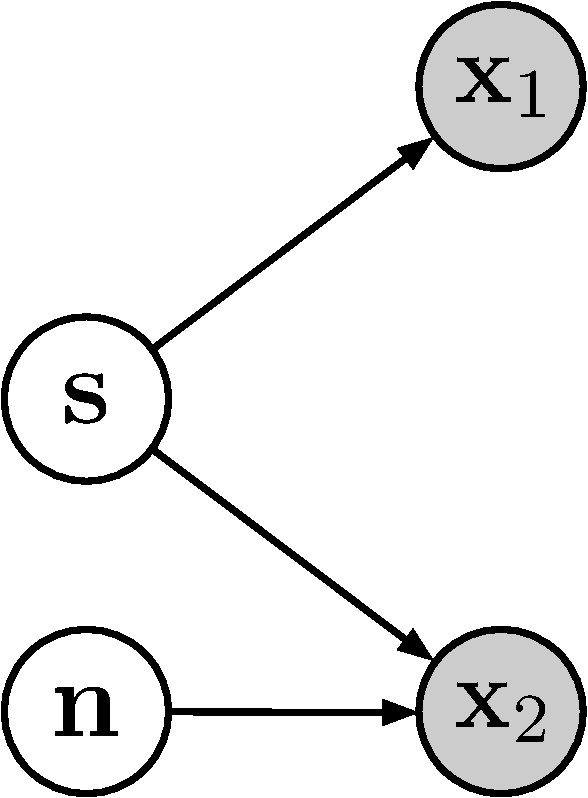
\includegraphics[scale=0.3]{img_pdf/one_noisy.pdf}
	\caption{The setting considered in Section \ref{sec:onenoisless}. Two views of the sources are available, one of which, $\bm{x}_1$, is not corrupted by noise. In this and all other figures, each node is a deterministic function of all its parents in the graph.
	}
	\label{fig:generalized_hsr_basic}
\end{figure}

\medskip

\begin{theorem}
	\label{thm:noiseless1}
	The difference between the log joint probability and log product of marginals of the observed variables in the model given in Equations \ref{eq:indep}-\ref{eq:sem2_1} admits the following factorisation:
	\begin{align}
	&\log p({x}_1, {x}_2) - \log p({x}_1) p({x}_2) \nonumber \\
	&= \log p({x}_2 | {x}_1) - \log p({x}_2) \nonumber\\
	&= \left(\sum_i \alpha_i(s_{i}, g_i(s_i, n_i)) + \log \det J \right) \nonumber\\
	&\qquad - \left( \sum_i \delta_i(g_i(s_i, n_i)) + \log \det J\right) \nonumber\\
	&= \sum_i \alpha_i(s_{i}, g_i(s_i, n_i)) - \sum_i \delta_i(g_i(s_i, n_i))\label{eq:logdens_noiesless_1} \,
	\end{align}
	where $s_i=f^{-1}_{1i}({x}_1)$, $g_i=f^{-1}_{2i}({x}_2)$,
	and $J$ is the Jacobian of the transformation $f^{-1}_2$ (note that the introduced Jacobians cancel\footnote{Several subsequent results in this section consider the difference between two log-probabilities.
In all of these cases, the Jacobians introduced by a change of variables cancel out as in Equation \ref{eq:logdens_noiesless_1}.
For brevity these Jacobians are omitted henceforth.}).
	Suppose that
	\begin{enumerate}
		\item $\alpha$ satisfies the \emph{Sufficiently Distinct Views} assumption (see after this theorem).
		\item A classifier is trained to discriminate between
		\begin{align*}
		(X_{1},X_{2}) \text{ vs. } (X_{1},X_{2}^{*})\,,
		\end{align*}
		where $({X}_{1},{X}_{2})$ correspond to the same realisation of $Z$ and $({X}_{1},{X}_{2}^{*})$ correspond to different realisations of ${Z}$.
		\item The classifier minimises the logistic regression loss, and is constrained to use a regression function of the form
		\begin{equation*}
		r({x}_{1},{x}_{2})=\sum_{i}\psi_{i}(h_{i}({x}_{1}),{x}_{2})
		\end{equation*}
		where ${h} =(h_{1}, \ldots, h_{n})$  is invertible, smooth and has smooth inverse.
	\end{enumerate}
	
	Then, in the limit of infinite data and with universal approximation capacity, $h$ inverts ${f}_1$ in the sense that the $h_{i}(X_1)$ recover the independent components of $Z$ up to component-wise invertible transformations.
\end{theorem}
An outline of the proof for this result is provided below after discussing some of the assumptions; full proof can be found in Appendix \ref{appendix:proof-thm1}.

The assumption of invertibility for $h$ could be satisfied by, e.g., the use of normalizing flows~\citep{rezende2015variational, chen2018neural} or deep invertible networks~\citep{jacobsen_hal-01712808}.


If $X_1$ and $X_2$ were always equal, the multiple view setting would reduce to the normal nonlinear ICA setting.
The \emph{Sufficiently Distinct Views (SDV)} assumption formalises a sense in which the two views must be sufficiently different from one another,
resulting in more information being available in totality than from each view individually.
In the context of Theorem~\ref{thm:noiseless1}, it is an assumption about the log-probability of the \emph{corruption} conditioned on the source.
Informally, it demands that the probability distribution of the corruption should vary significantly as a result of conditioning on different values of the source.

\medskip

\begin{definition}[Sufficiently Distinct Views]\label{suff_dist_assumption}
	Let $\alpha_i(y_i, t_i)$, $i=1,\ldots, N$ be functions of two arguments.
	Denote by $\alpha$ the vector of functions and define
	\begin{align}
	\alpha'_{i}(y_i, t_i)&= \partial \alpha_{i}(y_i, t_i)/\partial y_i, \label{eq:convention1}\\
	\alpha''_{i}(y_i, t_i)&=\partial^2 \alpha_{i}(y_i, t_i)/\partial y_i^2\, \label{eq:convention2}\\
	{w}_{\alpha}({y}, {t}) &= (\alpha''_{1}, \ldots, \alpha''_{D}, \alpha'_{1}, \ldots,\alpha'_{D}).
	\end{align}
	We say that ${\alpha}$ satisfies the assumption of \emph{Sufficiently Distinct Views (SDV)} if for any value of ${y}$, there exist $2D$ distinct values ${t}^j$, $j=1, \ldots, 2D$ such that the vectors ${w}({y},{t}^j)$ are linearly independent.
	\\    \end{definition}
This is closely related to the Assumption of Variability in~\cite{hyvarinen19a}.
The SDV assumption is discussed in further detail in Section \ref{appendix:sdv}, where simple cases of conditional log-probability density functions satisfying and violating the assumption are presented.

\begin{proof}[Sketch proof of Theorem \ref{thm:noiseless1}]
The first observation to be made is that for logistic regression, the optimal regression function for the logit $r(x_1, x_2)$ is equal to the log density-ratio between the two distributions being distinguished.
Thus, in the limit of infinite data and with universal approximation capacity, the following equality holds:
%
\begin{align*}
\sum_{i}\psi_{i}(h_{i}({x}_{1}),{x}_{2}) = \sum_i \alpha_i(s_{i}, g_i(s_i, n_i)) - \sum_i \delta_i(g_i(s_i, n_i)).
\end{align*}
%
By performing the change of variables $y=h(x_1)$, $t=f_2^{-1}(x_2)$, and defining $v(y) := f_1^{-1}(h^{-1}(y)) = s$, this equation can be rewritten
%
\begin{align}
\sum_{i}\psi_{i}(y_i,f_2(t)) = \sum_i \alpha_i(v_i(y), t_i) - \sum_i \delta_i(t_i). \label{eqn:ica-first-theorem-proof}
\end{align}
%
The goal is to show that $v_i(y)$ depends on exactly one coordinate of $y$, so that $v_i(y) = v_i(y_j)$ for some $j$. 
Since $s = v(y)$, this implies that $s_i = v_i(y_j)$ is a function only of $y_j$, which in turn implies that $s_i$ is a function only of $h_j(x_1)$. 
Since $v = f_1^{-1} \circ h^{-1}$ is the composition of two invertible functions, it is itself invertible, and since each component of $v$ depends only one one component of its input, each of the components are also invertible.
It follows that $s_i$ is an invertible function of $h_j(x_1)$, and so $h(x_1)$ recovers $s$ up to permutations and coordinate-wise invertible transformations.

Showing that $v_i(y) = v_i(y_j)$ for some $j$ is somewhat technically involved, and it is here that the SDV assumption is required.
It is proved by taking partial derivatives of Equation \ref{eqn:ica-first-theorem-proof} with respect to $y_i$ and $y_j$ for $j\not=i$. 
This results in an expression involving first- and second-order derivatives of $\alpha_i$ and $v_i$ in which the expressions in the SDV assumption appear. 
If the SDV assumption holds, it follows that the derivative of $v_i$ with respect to $y_j$ is everywhere zero, meaning that $v_i$ does not depend on $y_j$. 
See the full proof in Appendix \ref{appendix:proof-thm1} for further details.
\end{proof}

Theorem \ref{thm:noiseless1} shows that by jointly considering the two views, it is possible to recover $Z$, in contrast to the single-view setting.
This result can be extended to learn the inverse of ${f}_2$ up to component-wise invertible functions.

\medskip

\begin{corollary}
	\label{crl:noiseless1}
	Consider the setting of Theorem \ref{thm:noiseless1} with the alternative factorisation of the log joint probability
	\begin{align}
	&\log p({x}_1, {x}_2) - \log p({x}_1) p({x}_2) \nonumber \\
	&= \log p({x}_1 | {x}_2) - \log p({x}_1)\nonumber \\
	&= \sum_i \gamma_i(s_{i}, g_i(s_i, n_i)) - \sum_i \beta_i(s_i)) \label{eq:logdens_noiesless_2}\,.
	\end{align}
	Suppose that ${\gamma}$ satisfies the SDV assumption.
	Replacing the regression function with
	\begin{equation*}
	r({x}_{1},{x}_{2})=\sum_{i}\psi_{i}({x}_{1}, h_{i}({x}_{2}))
	\end{equation*}
	results in ${h}$ inverting ${f}_2$ in the sense that the $h_{i}({x}_2)$ recover the independent components of ${g}({s}, {n})$ up  to component-wise invertible transformations.
\end{corollary}
The proof is similar to that of Theorem \ref{thm:noiseless1} and can be found in Appendix \ref{appendix:proof-cor2}.
These two results together mean that it is possible to learn inverses ${h}_1$ and ${h}_2$ of ${f}_1$ and ${f}_2$, and therefore to recover ${s}$ and ${g}({s}, {n})$, up to component-wise intertible functions.
Note, however, that doing so requires running two separate algorithms.
Furthermore, there is no guarantee that the learned inverses ${h}_1$ and ${h}_2$ are `aligned' in the sense that for each $i$ the components ${h}_{1i}({x}_1)$ and ${h}_{2i}({x}_2)$ correspond to the same components of ${s}$.

This problem of misalignment can be resolved by changing the form of the regression function.

\medskip

\begin{theorem}\label{thm:demixing}
	Consider the settings of Theorem \ref{thm:noiseless1} and Corollary \ref{crl:noiseless1}.
	Suppose that both ${\alpha}$ and ${\gamma}$ satisfy the SDV assumption.
	Replacing the regression function with
	\begin{equation}\label{eqn:double-regression-fn}
	r({x}_{1},{x}_{2})=\sum_{i}\psi_{i}(h_{1,i}({x}_{1}),h_{2,i}({x}_{2}))
	\end{equation}
	results in ${h}_1$, ${h}_2$ inverting ${f}_1$, ${f}_2$ in the sense that the $h_{1,i}({x}_1)$ and $h_{2,i}({x}_2)$ recover the independent components of ${s}$ and ${g}({s}, {n})$ up to two different component-wise invertible transformations. Furthermore, the two representations are aligned, i.e. for $i\not=j$,
	\begin{equation*}
	h_{1,i}(\mathbf{x}_{1})\independent h_{2,j}(\mathbf{x}_{2})
	\end{equation*}
\end{theorem}
The proof is similar to that of Theorem \ref{thm:noiseless1} and can be found in Appendix \ref{appendix:thm1}.

Note that Theorem \ref{thm:demixing} is \emph{not} a generalisation of Theorem \ref{thm:noiseless1} or Corollary \ref{crl:noiseless1}, since it makes stricter assumptions by imposing the SDV assumption on both ${\alpha}$ and ${\gamma}$.
In contrast, Theorem \ref{thm:noiseless1} and Corollary \ref{crl:noiseless1} require that only one is valid for each.
For cases in which finding aligned representations for ${s}$ and ${g}({s}, {n})$ are desired, Theorem \ref{thm:demixing} should be applied.
If the only goal is recovery of ${s}$, the assumptions of Theorem \ref{thm:noiseless1} are easier to satisfy.


In practical applications, the multi-view scenario is useful in multimodal datasets where one of the two acquisition modalities has much higher signal to noise ratio than the other one (e.g., in neuroimaging, when simultaneous fMRI and Optical Imaging recordings are compared). In such cases, jointly exploiting the multiple modalities would help to discern a meaningful and identifiable latent representation which could not be attained through analysis of the more reliable modality alone.


%\subsubsection{Equivalence with Permutation Contrastive Learning for Time Dependent Sources}
%Note that the analysis of Theorem~\ref{thm:noiseless1} covers the case of temporally dependent stationary sources analyzed in~\cite{pmlr-v54-hyvarinen17a}.
%Indeed, if it is further assumed that $\bm{s}$ and $\bm{g}(\bm{s}, \bm{n})$ are uniformly dependent~\cite{pmlr-v54-hyvarinen17a}, they can be seen as a pair of subsequent time points of an ergodic stationary stochastic process for which the analysis of Theorem 1 of~\cite{pmlr-v54-hyvarinen17a} would hold. In other words, we can define a stochastic process as $p(\bm{s}_{t+1}| \bm{s}_t) := p(\bm{g}(\bm{s}, \bm{n})| \bm{s})$.
%Note that while the two formulations are theoretically equivalent, our view offers a wider applicability as it covers the asynchronous sensing of $\bm{s}$, provided that multiple measurements (i.e. $\bm{x}_1, \bm{x}_2$) are available; additionally, our \textit{Sufficiently Distinct Views} assumption does not necessarily imply uniform dependency. Furthermore, while~\cite{pmlr-v54-hyvarinen17a} considers a generative model of the form $\bm{x}(t) = \bm{f}(\bm{s}(t))$, thus constraining the mixing function to be the same for any two data points $\bm{x}(t_1)$, $\bm{x}(t_2)$, in our setting we consider two different mixing functions, $\bm{f}_1$ and $\bm{f}_2$, for the two different views.
%Finally, we study this setting as an intermediate step for the following two sections, in which no deterministic function of the sources is observed, learning to invert any of the $\bm{f}_i$ can only recover $\bm{s}$ up to the corruption operated by $\bm{g}$.

\subsection{Two noisy views}
\label{sec:constrained}

\begin{figure}[t!]
	\centering
	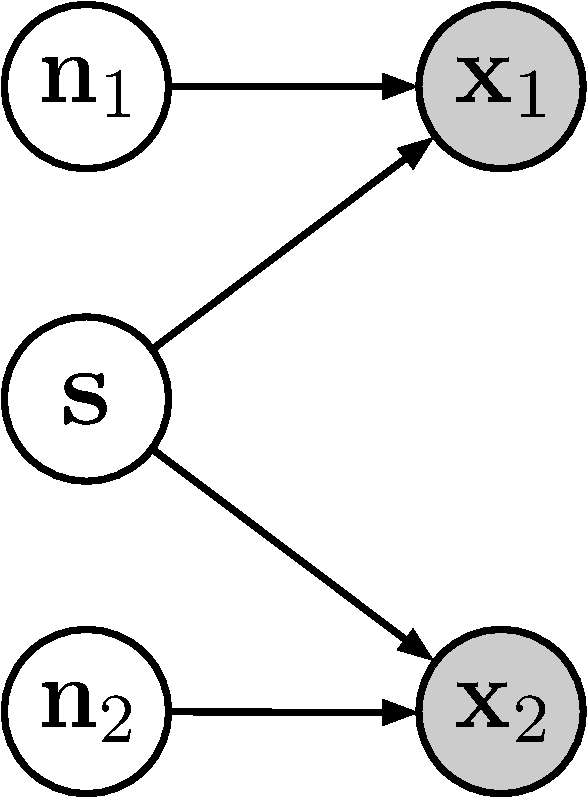
\includegraphics[scale=0.3]{img_pdf/classic_hsr.pdf}
	\caption{Setting with two views of the sources $\bm{s}$, both corrupted by noise.}
	\label{fig:classic_hsr}
\end{figure}

Consider next the setting in which both variables are corrupted by noise, depicted in Figure \ref{fig:classic_hsr} and described by the following model:
\begin{align*}
X_{1}&={f}_{1}({g}_{1}({Z},N_{1}))  \\
X_{2}&={f}_{2}({g}_{2}({Z},N_{2}))  \,,
\end{align*}
where all variables take value in $\mathbb{R}^D$, ${f}_{1}$ and ${f}_{2}$ are nonlinear, invertible, deterministic functions,
${g}_{1}$ and ${g}_{2}$ are component-wise corrupters, and $Z$ and the $N_i$ are independent with independent components.
This class of models generalises the setting of Section \ref{sec:onenoisless}, since by taking ${g}_1(Z, N_1) = Z$ it reduces to the case of one noiseless observation.

The log density ratio $\log p({x}_1, {x}_2) - \log p({x}_1)p({x}_2)$ admits similar factorisations to those given in Equations \ref{eq:logdens_noiesless_1} and \ref{eq:logdens_noiesless_2}:
\begin{align}
&\log p({x}_1, {x}_2) - \log p({x}_1) p({x}_2) \nonumber\\
&= \log p({x}_1 | {x}_2) - \log p({x}_1)\nonumber\\
&= \sum_i \eta_i(g_{1i}(s_i, n_{i1}), g_{2i}(s_i, n_{2i})) - \sum_i \theta_i(g_{1i}(s_i, n_{1i}) \label{eq:noisylogdens_1}\\
&= \log p({x}_2 | {x}_1) - \log p({x}_2) \nonumber\\
&= \sum_i \lambda_i(g_{2i}(s_i, n_{2i}), g_{1i}(s_i, n_{1i})) - \sum_i \mu_i(g_{2i}(s_i, n_{2i})) \label{eq:noisylogdens_2}
\end{align}
Since access is only given to corrupted observations, exact recovery of $Z$ is not possible.
Nonetheless, a generalisation of Theorem \ref{thm:demixing} holds showing that the ${f}_i$ can be inverted and $Z$ recovered up to the corruptions induced by the $N_i$ via the ${g}_i$.

\medskip

\begin{theorem}\label{thm:two-noisy-views}
	Suppose that ${\eta}$ and ${\lambda}$ satisfy the SDV assumption.
	The algorithm described in Theorem \ref{thm:noiseless1} with regression function specified in Equation \ref{eqn:double-regression-fn} results in ${h}_1$ and ${h}_2$ inverting ${f}_1$ and ${f}_2$ in the sense that the $h_{1,i}({x}_1)$ and $h_{2,i}(\bm{x}_2)$ recover the independent components of $\bm{g}_1(\bm{s}, \bm{n}_1)$ and $\bm{g}_2(\bm{s}, \bm{n}_2)$ up to two different component-wise invertible transformations. Furthermore, the two representations are aligned, i.e. for $i\not=j$,
	\begin{equation*}
	h_{1,i}(\mathbf{x}_{1})\independent h_{2,j}(\mathbf{x}_{2})
	\end{equation*}
\end{theorem}
The proof can be found in Appendix \ref{appendix:thm1}.




We can thus recover the common source $\bm{s}$ up to the corruptions $\bm{g}_i(\bm{s}, \bm{n}_i)$.
In the limit of the magnitude of one of the noise variables going to zero, the reconstruction of the sources $\sbm$ attained through the corresponding view is exact up to the component-wise invertible functions, as stated in the following corollary.

\medskip

\begin{corollary}
	\label{crl:lownoise}
	Let $\bm{n}_1^{(k)} = \frac{1}{k} \cdot  \Tilde{\bm{n}}$ for $k \in \NN$, where $\Tilde{\bm{n}}\in\mathbb{R}^D$ is a fixed random variable, and $\bm{n}_2$ be a random variable that does not depend on $k$.
	Let $\bm{h}_1^{(k)}, \bm{h}_2^{(k)}$ be the output of the algorithm specified by Theorem \ref{thm:two-noisy-views} with noise variables $\bm{n}_1^{(k)}$ and $\bm{n}_2$.
	
	Suppose that the corrupters $\bm{g}_i$ satisfy the following two criteria:
	\begin{enumerate}
		\item $\exists \bm{a}  \in \mathbb{R}_{> 0}^D \: $   s.t. $\: \left|\frac{\partial \bm{g}_1(\bm{s},\bm{n})}{\partial \bm{n}} \right|_{\bm{n}=0} \leq \bm{a} \: $ for all $\bm{s}$
		\item $\exists \bm{b}  \in \mathbb{R}_{> 0}^D \: $ s.t. $\: 0<\frac{\partial \bm{g}_1(\bm{s},0)}{\partial \bm{s}} \leq \bm{b}$
	\end{enumerate}
	Then, denoting by $\bm{E}$ the set of all scalar, invertible functions, we have that
	\[
	\lim_{k \to \infty} \inf_{\bm{e}\in \bm{E}} \left \|\bm{s} - \bm{e}(\bm{h}_1^{(k)}(\bm{x}_1)) \right \| = 0
	\]
\end{corollary}
The proof can be found in Appendix \ref{appendix:thm2}.

Corollary \ref{crl:lownoise} implies that in the limit of small noise, the sources $\bm{s}$ can be recovered exactly.
Condition \textit{1} upper bounds the influence of $\bm{n}$ on the corruption: we can not hope to retrieve $\bm{s}$ if $\bm{g}(\bm{s}, \bm{n})$ contains too little signal.
Condition \textit{2} ensures that the function $\bm{g}$ is invertible with respect to $\bm{s}$ when $\bm{n}$ is equal to zero.
If this were not satisfied, some information about $\bm{s}$ would be washed out by $\bm{g}$ even in absence of noise.
This would make recovery of $\bm{s}$ trivially impossible.


\subsection{Multiple noisy views}
\label{sec:multiple}

The results of Section \ref{sec:constrained} state that in the two noisy views setting, $\bm{s}$ can be recovered up to the corruptions.
In the limit that the magnitude of the noises goes to zero, the uncorrupted $\bm{s}$ can be recovered.
The intuition is that the less noise there is, the more information each observation provides about $\bm{s}$.

\begin{figure}[t!]
	\centering
	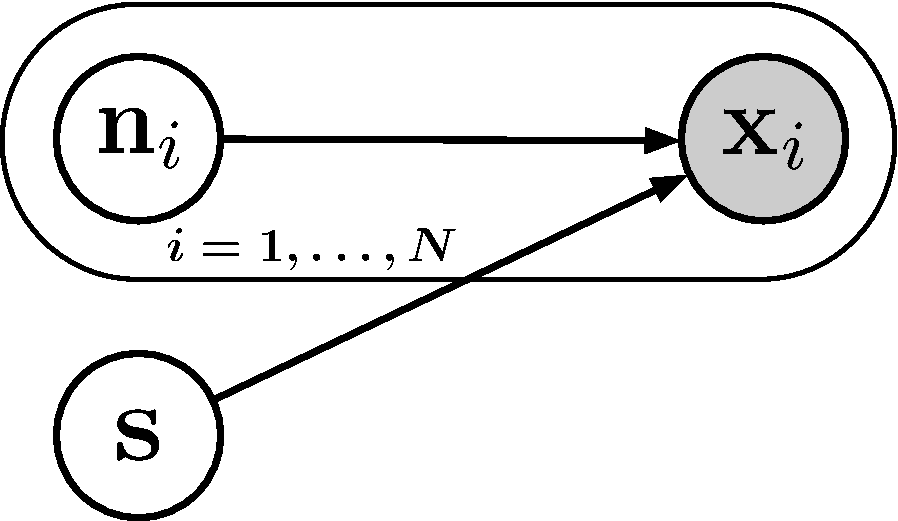
\includegraphics[scale=0.3]{img_pdf/generalized_hsr_many.pdf}
	\caption{Setting with $N$ corrupted views of the sources.}
	\label{fig:generalized_hsr_many}
\end{figure}

In this section we consider the multi-view setting, where $N$ distinct noisy views of $\bm{s}$ are available,
\begin{equation*}
\bm{x}_{i}=\bm{f}_{i}(\bm{g}_{i}(\bm{s},\bm{n}_{i}))\,\,\,,i=1, \ldots, N\,, \label{eq:multi}\\
\end{equation*}
and the noise variables $\bm{n}_{i}$ are mutually independent, as represented in Figure \ref{fig:generalized_hsr_many}.
Since each view provides additional information about $\bm{s}$, we ask: in the limit as $N \to \infty$, is it possible to reconstruct $\bm{s}$ exactly?


By applying Theorem \ref{thm:two-noisy-views} to the pair $(\bm{x}_1,\bm{x}_i)$ it is possible to recover  $(\bm{g}_1(\bm{s},\bm{n}_1),\bm{g}_i(\bm{s},\bm{n}_i))$ such that the components are aligned, but up to different component-wise invertible functions $\bm{k}_1$ and $\bm{k}_i$.
Running the algorithm on a different pair  $(\bm{x}_1,\bm{x}_{j})$ will result in recovery up to different component-wise invertible functions $\bm{k}'_1$ and $\bm{k}'_j$.

Note that these will \emph{not} necessarily result in  $\bm{k}_i\circ\bm{g}_i(\bm{s},\bm{n}_i)$ and $\bm{k}'_j\circ\bm{g}_j(\bm{s},\bm{n}_j)$ being aligned with each other.
However, the components of $\bm{k}_1\circ\bm{g}_1(\bm{s},\bm{n}_1)$ and $\bm{k}'_1\circ\bm{g}_1(\bm{s},\bm{n}_1)$ are the same, up to permutation and component-wise invertible functions.
This permutation can therefore be undone by performing independence testing between each pair of components.
Components that are `different' will be independent; those that are the same will be deterministically related.
Therefore, they can be used as a reference to permute the components of $\bm{k}'_j$ and make it aligned with $\bm{k}_i$.

The problem is then how to combine the information from each aligned $\bm{k}_i \circ \bm{g}_i(\bm{s},\bm{n}_i)$ to more precisely identify $\bm{s}$.
The fact that the components are recovered up to \emph{different} scalar invertible functions makes combining information from different views non-trivial.


As a first step in this direction, we consider the special case that each $\bm{g}_i$ acts additively and each $\bm{n}_i$ is zero mean and each of $\bm{s}$ and the $\bm{n}_i$ are independent with independent components.
\begin{align}
\left.
\begin{array}{ll}
&\bm{x}_{i}=\bm{f}_{i}(\bm{s} + \bm{n}_{i}) \\
&\mathbb{E}[\bm{n}_i]= 0
\end{array}
\right\rbrace \quad i \in \mathbb{N}
\end{align}

Suppose to begin with that we are able to recover each $\bm{s} + \bm{n}_i$ \emph{without} the usual component-wise invertible functions. Then, writing $\bm{n}$ to denote all of the $\bm{n}_i$, it is possible to estimate $\bm{s}$ as
\begin{align*}
\bm{s} \approx \Omega^N(\bm{s}, \bm{n}) = \frac{1}{N}\sum_{i=1}^N \left(\bm{s} + \bm{n}_i\right).
\end{align*}
Subject to mild conditions on the rate of growth of the variances $\text{Var}(\bm{n}_i)$ as $i\to\infty$, Kolmogorov's strong law implies that $\Omega^N(\bm{s}, \bm{n})$ is a good approximation to $\bm{s}$ as $N\to\infty$ in the sense that  $\Omega^N(\bm{s}, \bm{n}) \overset{a.s.}{\longrightarrow} \bm{s}$.
This implies moreover that it is possible to reconstruct the $\bm{n}_i$ by considering the residue $R^N_i(\bm{s}, \bm{n}) = (\bm{s} + \bm{n}_i) - \Omega^N(\bm{s}, \bm{n}) \overset{a.s.}{\longrightarrow} \bm{n}_i$.

In the presence of the unknown functions $\bm{k}_i$, we would be able to reconstruct $\bm{s}$ and the $\bm{n}_i$ if we were able to identify the inverses $\bm{e}_i = \bm{k}_i^{-1}$ for each $i$.
For any component-wise invertible functions $\bm{e}_i$, define
\begin{align*}
\Omega_{\eb}^N(\bm{s}, \bm{n}) &= \frac{1}{N} \sum_{i=1}^N \bm{e}_i\circ \bm{k}_i( \bm{s} + \bm{n}_i) \\
R_{\bm{e}, i}^N(\bm{s}, \bm{n}) &= \bm{e}_i\circ \bm{k}_i( \bm{s} + \bm{n}_i) - \Omega_{\bm{e}}^N(\bm{s}, \bm{n}).\\
\end{align*}
$\bm{e}_i$ is something we can choose and $\bm{k}_i(\bm{s}+\bm{n}_i) = \bm{h}_i(\bm{x}_i)$ is the output of the algorithm, and hence $\Omega_{\eb}^N(\bm{s}, \bm{n})$ and $R_{\bm{e}, i}^N(\bm{s}, \bm{n})$ are random variables with known distributions.
Subject to mild conditions, the dependence of these quantities on most or all of the $\bm{n}_i$ becomes increasingly small as $N$ grows and disappears in the limit $N\to\infty$.

\medskip

\begin{lemma}\label{lem:last-lemma}
	Suppose that the sequence $\mathbb{E}_{\bm{n}}[\Omega_{\eb}^N(\bm{s}, \bm{n})] = \frac{1}{N}\sum_{i=1}^N \mathbb{E}_{\bm{n}_i}[\bm{e}_i\circ \bm{k}_i( \bm{s} + \bm{n}_i)] $ converges as $N \to \infty$ for almost all $\bm{s}$, and write this limit as
	\begin{align*}
	\Omega_\eb(\bm{s}) = \lim_{N\to\infty}\mathbb{E}_{\bm{n}}[\Omega_{\eb}^N(\bm{s}, \bm{n})].
	\end{align*}
	
	Suppose further that there exists $K$ such that $V_{\eb_i} = \mathrm{Var}\left(\bm{e}_i \circ \bm{g}_i(\bm{s} + \bm{n}_i) \right) \leq K$ for all $i$.
	Then
	\begin{align*}
	\Omega_{\eb}^N(\bm{s}, \bm{n}) & \overset{a.s.}{\longrightarrow} \Omega_{\eb}(\bm{s}) \\
	R_{\eb, i}^N(\bm{s}, \bm{n}) & \overset{a.s.}{\longrightarrow} R_{\eb, i}(\bm{s}, \bm{n}_i) = \bm{e}_i\circ \bm{k}_i( \bm{s} + \bm{n}_i) - \Omega_{\eb}(\bm{s})
	\end{align*}
\end{lemma}

The proof can be found in Appendix \ref{appendix:last-lemma}.
Given some choice of $\bm{e}$, we can think of $\Omega_{\eb}(\bm{s})$ and $R_{\eb, i}(\bm{s}, \bm{n}_i)$ as our putative candidates for $\bm{s}$ and $\bm{n}_i$ respectively.
As discussed earlier, if we could identify $\bm{e}_i=\bm{k}_i^{-1}$, then we would have $\Omega_{\eb}(\bm{s}) = \bm{s}$ and $R_{\eb, i}(\bm{s}, \bm{n}_i) = \bm{n}_i$, and thus $\Omega_{\eb}$ and $R_{\eb, i}$ would satisfy the same independences and other statistical properties as $\bm{s}$ and $\bm{n}_i$ respectively.
Can we use these properties as criteria to identify good choices of $\bm{e}_i$?

The following theorem gives a set of sufficient conditions under which each $\bm{e}_i$ inverts $\bm{k}_i$ up to some affine ambiguity which is the same for every $i$.

\medskip

\begin{theorem}
	\label{thm:lastthm}
	Suppose there exists $C>0$ such that $\text{Var}(\bm{n}_i) \leq C$ for all $i$ and let $\mathcal{G}_K = \big\lbrace
	\{\bm{e}_i \}$ s.t.
	\begin{align}
	& V_{\bm{e}_i} \leq K \ \forall i \label{eq:resid_1}\\
	& \Omega_{\bm{e}}(\bm{s}) < \infty \  \text{ for almost all } \bm{s} \label{eq:resid_2}\\
	&R_{\bm{e}, i} \independent R_{\bm{e}, j} \ \forall i \not= j, \label{eq:resid_3}\\
	\\    &\mathbb{E} R_{\bm{e}, i} = 0 \ \forall i \label{eq:resid_5} \\
	&R_{\bm{e}, i}(\bm{s}, \bm{n}_i) = R_{\bm{e}, i}(\bm{n}_i) \ \forall i \ \big\rbrace \label{eq:resid_6}
	\end{align}
	
	Then,
	\begin{align*}
	\mathcal{G}_K \subseteq\left\lbrace \{ \bm{\alpha} \bm{k}^{-1}_i + \bm{\beta} \} \ : \ \bm{\alpha} \in \mathbb{R}^{D}_{\not=0}, \: \bm{\beta} \in \mathbb{R}^{D} \right\rbrace
	\end{align*}
	where $\bm\alpha \bm{k}^{-1}_i$ denotes the element-wise product with the scalar elements of $\bm{\alpha}$.
	If $K \geq \text{Var}(\bm{s}) + C$, then $ \{ \bm{k}^{-1}_i \}  \in \mathcal{G}_K$,
	and so $\mathcal{G}_K$ is non-empty for $K$ sufficiently large.
\end{theorem}
The proof can be found in Appendix \ref{sec:lasttmpr}.
It follows that it is possible recover $\bm{s}$ and $\bm{n}_i$ up to $\bm{\alpha}$ and $\bm{\beta}$ via $\Omega_\eb(\bm{s}) = \bm{\alpha}\bm{s} + \bm{\beta}$ and $R_{\bm{e}, i}(\bm{n}_i) = \bm{\alpha}\bm{n}_i$.

We remark that each of the conditions \ref{eq:resid_1}--\ref{eq:resid_5} can be verified from known information.
We conjecture that condition \ref{eq:resid_6} can be relaxed to assuming the verifiable condition of independence between $\Omega_{\eb}(\bm{s})$ and $R_{\eb, i}(\bm{s}, \bm{n}_i)$ for all $i$ along with additional regularity assumptions on the functional form of $R_{\eb, i}$ (e.g. smoothness).

To conclude, Theorem 8 provides sufficient conditions under which it is possible to fully reconstruct $\bm{s}$ with corrupted views.
In contrast to previous results in Sections \ref{sec:onenoisless} and \ref{sec:constrained}, this result leverages infinitely many corrupted views rather than vanishingly small corruption of finitely many views.







\section{Discussion about assumptions}
\subsection{Classification and stochasticity}
\label{sec:converged}
Suppose that a variable $X$ is drawn with equal probability from two distributions $P_0$ and $P_1$ with densities $p_0(x)$ and $p_1(x)$ respectively.
A classifier $D: x \mapsto [0,1]$ is trained to estimate the posterior probability that a particular realisation of $X$ was drawn from $P_0$ with the cross entropy loss, i.e. the parameters of $D$ are chosen to minimise

\[
L(D) = \mathbb{E}_{X\sim P_0} \left[ - \log D(X) \right] + \mathbb{E}_{X\sim P_1} \left[ - \log (1 - D(X)) \right].
\]

As shown in, for instance, \cite{goodfellow2014generative}, the global optimum of this loss occurs when $D(x) = \frac{p_0(x)}{p_0(x) + p_1(x)}$, which can be rewritten as

\begin{align}
D(x) &= \frac{1}{1 + p_1(x)/p_0(x)}\\
&= \frac{1}{1 + \exp ( - \log (p_0(x)/p_1(x))) } \label{eq:density-ratio-classification}
\end{align}

Recall that in the setting we consider, the function $r(x_1, x_2)$ is trained to classify between the two cases that $(x_1, x_2)$ is drawn from the joint distribution $\mathbb{P}_{x_1, x_2}$ (\emph{class $0$}) or the product of marginals $\mathbb{P}_{x_1}\mathbb{P}_{x_2}$ (\emph{class $1$}).
$r(x_1, x_2)$ is trained so that $\frac{1}{1 + \exp(-r(x_1, x_2))}$ estimates the posterior probability of $(x_1, x_2)$ belonging to class 0.
By comparing to Equation \ref{eq:density-ratio-classification}, it can be seen that

\begin{align*}
r(x_1, x_2) &= \log \left( p(x_1, x_2) / p(x_1) p(x_2)\right) \\
&= \log p(x_1 | x_2)  - \log p(x_1) \\
&= \log p(x_2 | x_1)  - \log p(x_2) \\
\end{align*}

Note that in order for the classification trick of contrastive learning to be useful, the variables $x_1$ and $x_2$ cannot be deterministically related.
If this is the case, the log-ratio is everywhere either $0$ or $\infty$ and hence the learned features are not useful.

To see why this is the case, suppose that $x_1$, and $x_2$ are each $N$-dimensional vectors.
If they are deterministically related, $p(x_1, x_2)$ puts mass on an $N$-dimensional submanifold of a $2N$-dimensional space.
On the other hand, $p(x_1)p(x_2)$ will put mass on a $2N$-dim manifold since it is the product of two distributions each of which are N-dimensional.

In this case, the distributions $p(x_1, x_2)$ and $p(x_1)p(x_2)$ are therefore not absolutely continuous with respect to one another and thus the log-ratio is ill-defined: $p(x_1, x_2)/p(x_1)p(x_2) = \infty$ at any point $(x_1,x_2)$ at which $p(x_1, x_2)$ puts mass and zero at points where $p(x_1)p(x_2)$ puts mass and $p(x_1,x_2)$ does not.

It follows that the contrastive learning technique as used in the theorems considered in this chapter can only be applied when the different views $\bm{x}_1$ and $\bm{x}_2$ are not deterministically related.
It is for this technical reason that the corruptions are necessary.


\subsection{The sufficiently distinct views assumption}
\label{appendix:sdv}

We give the following two examples to provide intuition about the Sufficiently Distinct Views (SDV) assumption - one regarding a case in which it does not hold, and another one in which it does.


A simple case in which the assumption does not hold is when the conditional probability of $\bm{z}$ given $\bm{s}$ is Gaussian, as in

\begin{equation}
p(\bm{z}|\bm{s}) = \frac{1}{Z} \exp\left[ -\sum_i (z_i - s_i)^2/(2\sigma_i^2) \right]\,, \label{eq:unsatisfied}
\end{equation}

where $Z$ is the normalisation factor, $Z = (2\pi)^{n/2}  \prod_i \sigma_i$.
Since taking second derivatives of the log-probability with respect to $s_i$ results in constants,
it can be easily shown that there is no way to find $2D$ vectors $\bm{z}_j$, $j=1, \ldots, 2D$, such that the corresponding $\bm{w}(\bm{s}, \bm{z}_j)$ (see Definition 1) are linearly independent.


The fact that the assumption breaks down in this case is reminiscent of the breakdown in the case of Gaussianity for linear ICA. Interestingly, in our work, the true latent sources \textbf{are} allowed to be Gaussian. In fact, the distribution of $\bm{s}$ does not enter the expression above.


An example in which the SDV assumption does hold is a conditional pdf given by

\begin{equation}
p(\bm{z}|\bm{s}) = \frac{1}{Z(\bm{s})} \exp \left[ - \sum_i (z_i^2  s_i^2 + z_i^4 s_i^4  ) \right]\,, \label{eq:satisfied}
\end{equation}

where $Z(\bm{s})$ is again a normalisation function.
Proving that this distribution satisfies the SDV assumption requires a few lines of computation.
The idea is that $\bm{w}(\bm{s}, \bm{z})$ can be written as the product of a matrix and vector which are functions only of $\bm{s}$ and $\bm{z}$ respectively.
Once written in this form, it is straightforward to show that the columns of the matrix are linearly independent for almost all values of $\bm{s}$ and that $2D$ linearly independent vectors can be realised by different choices of $\bm{z}$.


\section{Conclusion}
\label{sec:on_suffistv}
We presented identifiability results in a novel setting by extending the formalism of nonlinear ICA.
We have investigated different scenarios of multi-view latent variable models and provided theoretical proofs on the possibility of inverting the mixing function and recovering the sources in each case.
Our results thus extend the scarce literature on identifiability for nonlinear ICA models.

In the classical noiseless ICA setting, the deterministic relationship between the sources and observations means that inverting the mixing function and recovering the sources are equivalent.
In contrast, we consider views of corrupted versions of the common sources, resulting in the decoupling of the demixing and retrieval of the sources.
Remarkably, Theorem \ref{thm:lastthm} points towards the possibility of simultaneously solving the two problems in the limit of infinitely many views.

Classical nonlinear ICA is provably non-identifiable because a single view is not sufficiently informative to resolve non-trivial ambiguities when recovering the sources.
While many papers in the ICA literature have explored placing restrictions either on the source distribution or on the form of the mixing to resolve these ambiguities, in this paper we consider exploiting additional views to constrain the inverse problem.
Clearly, if a second view is identical to the first, then nothing is gained by its observation.
Hence, in order for the second view to assist in resolving ambiguity, it must be sufficiently different from the first.
This is the intuition behind the technical assumption of \emph{sufficiently distinct views}.


Typically, noise is a nuisance variable that would be preferably non-existent.
In our setting, however, the noise variables acting on the sources are a crucial component, without which the contrastive learning approach could not be applied.
Furthermore, the assumption of sufficiently distinct views is ultimately an assumption about the complexity of the joint distribution of the (corrupted) sources corresponding to each view.
Without the noise variables the sufficiently distinct views assumption could not hold.


Our setting is relevant in a number of practical real-world applications, namely in all datasets that include multiple distinct measurements of related phenomena.
In practice, it may be better to think of the noise variables rather as intrinsic sources of variability specific to each view.
In most practical applications this would probably not be a significant limitation due to the prevalence of stochasticity in real-world systems.

An exemplary application of our method can be found in the field of neuroimaging.
Consider a study involving a cohort of subjects (perceivers), measuring their response to the presentation of the same stimulus.
One of the key problems in the field is how to extract a shared response from all subjects despite high inter-subject variability and complex nonlinear mappings between latent source and observation~\cite{chen2015reduced, haxby2011common}.
Our results provide principled ways to extract and decompose the components of the shared response.
In particular, the setting described in our model is suited to account for the high variability of the responses throughout the cohort, since the measurement corresponding to each subject is given by a combination of individual variability and shared response.

Looking to the future, we note that Theorem \ref{thm:lastthm} builds on the setting of Theorem \ref{thm:two-noisy-views} which only makes use of pairwise information from the observations.
A natural extension of this work should investigate algorithms that explicitly make use of $N>2$ views, which we conjecture would allow relaxation of the additivity assumption on the corruptions.
Furthermore, Theorem \ref{thm:lastthm} provides results that only hold for the asymptotic limit as the number of views becomes large.
Other extensions to this result could include analysis of the case of finitely many views.





